\chapter{Evaluation} \label{chap:system_archi}
This chapter describes the evaluation method and metrics used to measure the performance of the models. Additionally to validate the results of the Machine Learning models, a semi-structured interview conducted with the members of the marketing and sales team validates the significance of the approach used in this work. 
\section{Methods} \label{sect:thefirst}
To measure the performance of a machine learning based application there are certain metrics defined which indicates how well the the machine learning model has been trained. For example in a image classification problem, evaluation metrics such as precision, recall, F1 score, accuracy are used to denote how well the application can recognise a particular image. Similarly, there are some evaluation metrics defined that can be utilized to measure the performance of machine learning based recommender system. Furthermore such metrics also aid in selecting the appropriate algorithm.  \\ \par


The most common evaluation strategy used when deploying the recommender system in real-world environment consist of two methods namely: Online evaluation and Offline Evaluation.
\begin{itemize}
	\item \textit{Online Evaluation}\\
	 It helps in measuring the performance of the recommender system in real-life situations where the users interact with the system. One such way of implementing online evaluation is through A/B testing. Typically, A/B testing involves serving a fraction of random users with recommendations generated from recommender system A and another fraction with recommender system B. A utility function such as Click Through Rate (CTR) is then used which indicates which recommender system is more successful in attracting the user or capturing his interest. The results from such experiments helps in further fine tuning the algorithm to obtain the desired level of performance. Although Online evaluation techniques are useful, they require meticulous planning. Moreover, the cost associated with conducting such experiments are usually high owing to the significant investment in terms of resources, money and time \autocite[2941]{gunawardana2009survey}. Implementing an Online Evaluation experiments is out of scope of this study and hence has been excluded.
	\item \textit{Offline Evaluation}
	In most of the cases Online Evaluation is followed after Offline evaluation process. This is mainly because of the costs associated with Online Evaluation as well as to avoid any undesirable experience for the users of the system. Offline Evaluation provides the necessary experimentation setup for implementing different algorithm and testing it to achieve the desired level of performance. Recently there has been tremendous development in the algorithms for recommender systems suitable for a particular task. Offline evaluation setup exclude other algorithms and retain only those which showcase promising results which can be further extended to the Online evaluation phase thus reducing the risk of failure in later stages \autocite[2941]{gunawardana2009survey}. Offline evaluation tries to mimic the real-world environment by using the user-item interaction data-set similar to that of real-world deployment. In most of the scenarios the user-item interaction data-set refers to the past transactions, historical data related to the user,items and ratings. Depending on the underlying task of the recommender system i.e either to predict the ratings for unknown items for user or recommendations, the approach for training the machine learning model changes. In traditional machine learning problem, the data-set is divided into training data and testing data, where patterns are learned from the training set and are evaluated on the testing set. In recommender system following similar approach will lead to creating a bias, as some part of the data-set is not used leading to incorrect learning patters. One such strategy especially adopted while training machine learning models used in recommender systems is to mask certain percentage of the user-item interaction data to create the training data-set while the original data-set can be used as the testing data-set.
	
\end{itemize}


Since the development of recommender system is based on the tasks such as Ratings Prediction, Recommending Good items, or Optimizing some utility function \autocite[2938]{gunawardana2009survey}, the selection of the evaluation metric is specific to the task. The following section elaborates more on the metrics used specifically for recommender systems.

\section{Metrics}
As mentioned before the typical task associated with recommender system is either to Predict the ratings or to recommend some items. When evaluating recommender system the choice of evaluation metric is also dependent on factors such as the expected tasks, type of data (implicit or explicit) that is available for learning the machine learning models. As a result not all metrics can be used to measure the performance of the algorithm. Literature suggests that the metrics can be broadly divided into three categories Error based metrics, Accuracy based metrics, and Ranking based metrics as seen in table \ref{table:1}.  \\

\begin{table}[h!]
\centering
\begin{tabular}{|c| c| c|} 
 \hline 
 No. & Metric & Category\\ [0.5ex] 
 \hline \hline
 1 & Root Mean Squared Error (RMSE) & Error based \\ 
 \hline
 2 & Mean Squared Error (MSE) & Error based \\ 
 \hline
 3 & Mean Absolute Error (MAE) & Error based \\ 
 \hline
 4 & Mean Average Precision (MAP) & Accuracy based \\ 
 \hline
 5 & Mean Average Recall (MAR) & Accuracy based \\
 \hline
 6 & Mean Reciprocal Rank (MRR)  & Rank based \\ 
 \hline
 7 & Normalized Discounted Cumulative Gain (NDGC) & Rank based \\ 
 \hline
\end{tabular}
\caption{Categorization of evaluation metrics}
\label{table:1}
\end{table}

\begin{itemize}
	\item \textit{Error based metrics}: Typically used when a rich data-set containing explicit ratings for items is available and we want to predict the ratings for the items which were not rated by the user. Metrics such as Root Mean Squared Error (RMSE), Mean Squared Error (MSE), Mean Absolute Error(MAE) are often used in such scenario. 
	\item \textit{Accuracy based metrics}: These metrics are useful in determining the relevancy of the recommendations generated for the users. Inspiration on the usage of such metrics is drawn from the Information Retrieval domain, where the objective is to retrieve information within documents or retrieving relevant documents to a given query. Similarly, in recommender systems given the set of interactions between users and items, the recommender system should be able to recommend items that may be relevant to the user. Using this understanding, we can construct the basic structure for the evaluation. One such construct is \textit{confusion matrix} as show in Fig \ref{fig:confusion_matrix}, where each row in the matrix represents the outcome of the recommender system and the columns represent the actual observed interaction between user and item. Since this study is based on implicit feedback data represented in binary format i.e. if a user preferred an item or not, accuracy based evaluation metrics are more suitable for evaluating algorithm performance. Some of the most commonly used metrics are Mean Average Precision (MAP@K), Mean Average Recall(MRR@K).
	
	\item \textit{Rank based metrics}: Such metrics are used when the ranking is of importance in the top-k results generated by the recommender system. The most commonly used metrics are Normalized Discounted Cumulative Gain (NDGC), Mean Reciprocal Rank (MRR)
\end{itemize} \\
\par

In this study, the task of the recommendation of the items is the main focus.  This task is binary in nature, i.e. 0 dislike and 1 like. Accuracy based metrics namely Mean Average Precision (MAP) and Mean average Recall (MAR) used to evaluate the machine learning model. Root Mean Squared Error is one of the popular method used for assessing an algorithm. However, such metrics are useful when the task of predicting the ratings is performed. The equation for calculating MAP@k and MAR@k is given in Equation \ref{eqn:MSE} and Equation \ref{eqn:RMSE} respectively where k represents the cutoff of items. \\
\par

\begin{equation}
\label{eqn:MSE} MAP @ k =    \frac{1}{|U|} * \sum\nolimits_{1}^{l} \textit{P}_u(k) . \textit{rel}_u(k) 
\end{equation}
 where:
    \begin{conditions}
     P_u(k)    &  Precision for user \textit{u} at k.\\   
     \textit{rel}_u(k) & it is just an indicator which says if the k^th item was relevant or not \\ 
     |U| & represents all users. \\ 
    \end{conditions}
\\


\begin{equation}
\label{eqn:RMSE} MAR @ k =    \frac{1}{|U|} * \sum\nolimits_{1}^{l} \textit{R}_u(k) . \textit{rel}_u(k) 
\end{equation}
where:
    \begin{conditions}
     R_u(k)    &  Recall for user \textit{u} at k.\\   
     \textit{rel}_u(k) & it is just an indicator which says if the k^th item was relevant or not \\ 
     |U| & represents all users. \\ 
    \end{conditions}
\\
\begin{figure}
    \centering
    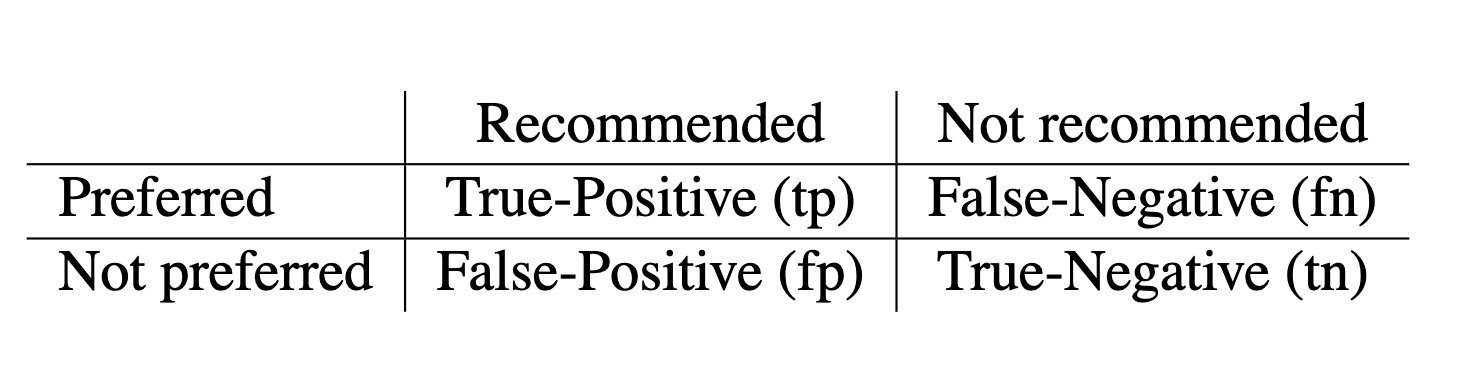
\includegraphics[scale=0.5]{chapters/figures/confusion_matrix.png}
    \caption{Representation of Recommender System result in the form of Confusion Matrix. \\
    Source: In \autocite[2945]{gunawardana2009survey}}
    \label{fig:confusion_matrix}
\end{figure}
The precision \textit{P}\textsubscript{k} and recall \textit{R}\textsubscript{k} is calculated using the confusion matrix shown in Fig \ref{fig:confusion_matrix}. Precision and Recall is calculated by using Equation \ref{eqn:precision} and \ref{eqn:recall} respectively.

\begin{equation}
\label{eqn:precision} P =    \frac{tp}{tp+fp} .  
\end{equation}
where:
    \begin{conditions}
     tp    &  Represents the count of recommended and preferred items.\\   
     fp & Represents the count of recommended but not preferred items \\ 
     \end{conditions}

\begin{equation}
\label{eqn:recall} R =    \frac{tp}{tp+fn} .  
\end{equation}
where:
    \begin{conditions}
     tp    &  Represents the count of recommended and preferred items.\\   
     fn & Represents the count of not recommended but preferred items \\ 
     \end{conditions}



\section{Qualitative Interviews}
Qualitative study seeks to explain as much as precisely as possible the social environment of people , communities and societies as its members experience it or live it. The exploratory nature of the Qualitative research allows the researchers to understand and explain certain behavior or an event \autocite[52]{demarrais2004qualitative}. The most common form of conducting Qualitative research is via Interviews. For \textcite[54]{demarrais2004qualitative}
interview means a conversation between the researcher and the participant where questions which elicit the participants opinions, perspectives related to the research study are asked. According to \textcite[251]{britten1995qualitative} Qualitative Interviews can be classified into three categories namely: Structured, Semi-structured, Unstructured or Depth. They are described as follows.
\begin{itemize}
    \item \textit{Structured Interview}: Such interview are based on fixed set of questions which are asked in the same order to each of the participant with no flexibility to ask follow-up or probing questions \autocite[65]{fylan2005semi}. For e.g. A questionnaire consisting of closed ended questions (yes/no types) which are read out to the participants and their response is documented.  Due to its structured nature, systematic collections of data is facilitated. Although Structured interview may result quick, better and well founded results, it may miss out on critical detailed information.
    
    \item \textit{Semi-structured Interview}: Unlike structured interview, semi-structured interview does not have any fixed set of questions but it usually consist of simple and open ended questions (interview guideline) related to the area of research \autocite[65]{fylan2005semi}. Thus combining the both open and closed ended questions. For e.g. Why and How type questions related to the research area along with follow-up for probing questions. Since this type of interview gives some flexibility to ask questions, detailed information is collected.
    
    \item \textit{Unstructured/Depth}: These interviews are less structured than semi-structured interviews where the focus is on few research topics which are explored in detail via open ended questions\autocite[251]{britten1995qualitative}. Lack of structure also means that the researcher must drive and control the direction of the interview. The researcher must have good knowledge of the area of the research. Because of its unstructured nature, the interview may be lengthy.
\end{itemize}

\textcite[65]{fylan2005semi} in her research states that Semi-structured interview are suitable when the aim of the research is to investigate rather than quantify. Additionally, such approach also helps the researcher to gain understanding of topic related to the research question and gain insight. Since the main theme of this study focus on the use of Recommender System in the context of Hyper-personalization and Digital Sales Excellence, it would be preferred to investigate what factors are important and for what reasons. By interviewing the members from the Sales and Marketing department at RTI Sports insights on the topic of using data driven process in deriving sales and marketing strategies will be helpful. Considering these criteria, a semi-structured interview type is more suitable for this work.  \\
\par
Preparing a Qualitative Interview involves series of steps that needs prior preparation. Overall the process of planning and conducting the semi-structured interview involves several steps and they are elaborated as follows
\begin{itemize}
    \item \textit{Designing the interview}:The first step i.e. designing the interview is crucial and leads to setting the right tone for the interview. According to \textcite[59]{demarrais2004qualitative} the interview must be designed keeping in mind the research questions. Also considering the semi-structured interview style, a interview guideline is handy and helps the researcher to keep the interview on track. As per \textcite[61]{demarrais2004qualitative} the interview guide should include questions which are short, clear to understand and result in detailed response. Additionally, the questions should also prompt the users to narrate their past experience or an event. The interview guideline should also include probing or follow up questions to get more detailed response from the participant.
    
    \item \textit{Selecting Participants}
    As \textcite[68]{fylan2005semi} suggests, the researcher must select the right participants who are keen to participate in the interview. There are many methods through which a researcher can sample the participants for the interview. One such method is purposive sampling technique \autocite[68]{fylan2005semi}. Purposive sampling method emphasises on selecting participants who are expert and knowledgeable in their respective fields. Keeping in mind the focus of this work, candidates with background in sales and marketing department are shortlisted. 
    
    \item \textit{Conducting interview}: As discussed earlier, semi-structured interview are conducted with the help of a interview guideline. Therefore preparing a well thought interview guideline is important. Apart from that other practical aspects associated with the interview should also be taking into consideration. Aspects such as interview mode, location, equipment's required etc. Interviews can be conducted in different ways. They can either be in person, via video conference applications such as Skype or telephonic way depending on the agreement with the participants \autocite[248]{luo2009semistructured}. If conducting the interview in person then it is good to arrange the chairs and table to make the participant comfortable \autocite[69]{fylan2005semi}. In case of telephonic interview recording equipment must be checked for its proper functionality \autocite[69]{fylan2005semi}. \textcite[252]{luo2009semistructured} illustrates the general process of interview which begins with the introduction of the researcher, the purpose of the interview as well as obtaining prior consent for recording the conversation and using personal details. Following the introduction, the researcher can engage in a friendly conversation to create an comfortable environment. Using the interview guideline the researcher can drive the interview and try to initiate response from the participant. On covering the desired areas covered in the interview guideline, the researcher can conclude the interview by thanking the participant for their time.
    
    \item \textit{Analysis} The final part in the interview process is to analyse the data collected. Researchers can either record the conversation or take notes during the interview. \textcite[253]{britten1995qualitative} suggests that its better to record the interview than taking notes as it might interfere with the process of interview. Moreover, there are chances that minute details might be left out while taking notes. Transcribing the recorded interview is essential as it forms the basis for the further analysis of the data. Transcription is time-consuming process and the researchers must invest a considerable amount of time \autocite[253]{britten1995qualitative}. \textcite[252]{luo2009semistructured} also suggests transcribing parts of the interview in the interest of time and efforts required. Although, during analysis if some part are unclear then the original recording can always be referred. On transcribing the interviews, the appropriate a 
    
\end{itemize}


\subsection{Interview Guideline and Choice of Interview Partners}
The interview guideline provides the necessary guidance to the researcher during the interview \autocite[65]{fylan2005semi}. Additionally, the design of the interview guideline must consider the research questions formulated for the study. \textcite[106]{longhurst2003semi} suggests, the foremost task for the researchers is to make themselves fully aware about the topic of the study. Following that, a list of themes related to the study is identified which can be referred to form the questions. Researchers usually keep simple questions in the beginning to build up the rapport. As the conversation builds up the questions asked can be more specific to the themes to elicit the response from the participant. Although there is no strict order in which the questions should be asked, \textcite[107]{longhurst2003semi} suggest to follow the natural conversational flow.\\ 
\par Based on these suggestions, a interview guideline consisting of main theme is designed. The questions included focused on the understanding the pain-points in the existing sales process, its effect on the relationship with the dealers and how recommender systems will help to overcome the challenges. The interview guideline can be found in appendix. \\ 
\par
Apart from the well designed interview guideline the choice of the interview candidates is also crucial for the study.As this study is more focused towards the Marketing and Sales, and Machine learning field, candidates who have experience in either of these mentioned field were shortlisted. This deliberate way of selecting interview candidates is described as purposive sampling \autocite[68]{etikan2016comparison}. By doing so the researcher can derive information from the experience of the candidates. Therefore, candidates from the Marketing and Sales department were selected for interviews.

\subsection{Overview of Interview Conducted}
Overall six participants were interviewed in this study. The selected participants have strong work experience in the field of marketing and sales. Prior to the interview, the participants were asked for an appointment for around 30 minutes. The interview with all of the participants were conducted via telephone. On an average the interview lasted for around 35minutes.The interviews were conducted in English language and followed the interview guideline as discussed in the previous section. Although it was intended to touch all the topics of interest related to this study but it was followed entirely keeping in mind the flexibility associated with the semi-structured interview.  Transcription of the interview is attached in the appendix section. \\ 
\par
The interview started with greeting the participants and introducing them to the topic. Participants were also notified about the purpose of the interview during scheduling the appointment. Out of total 6 participants, 2 participants denied the consent to mention their name in the transcription. Therefore their names are not included in the transcription and is represented by ND (not defined). After this the initial questions were related to their role in the organization. To which all of the participants are from the Marketing and Sales department and have an experience in the range of 3-15 years.The next question was asked With an intention to understand their responsibilities and roles specifically related to the Marketing department. Follow up question related to their response were asked specifically to the tools/applications that are used in the current scenario. Furthermore, the next question were asked to understand the experience with respect to the e-commerce applications that use active Recommender System for e.g. Amazon, eBay. Follow up question related to understand if they had any wow or surprising moment with such applications. Gradually the questions asked were more specific to the sales process, problems with it and use of recommender system to resolve them. The interview concluded with an open question if the participant had any comment, question related to the study followed by a thanking note for their participation. 

\section{Qualitative Content Analysis of the Interviews}
Qualitative content analysis is the main part in the qualitative study. The interviews conducted and its transcription leads to a lot of unstructured content which needs to be analysed. A qualitative analysis of such content leads to a better understanding of the main theme from the experiences of the participating candidates \autocite[10]{bengtsson2016plan}. Furthermore, \textcite[3]{mayring2014qualitative} proposed procedures of qualitative content analysis namely: Inductive category development and Deductive Category application. Since this study is based on the thematic analysis, Deductive category application procedure is more suitable for the content analysis. The procedure, consist of assigning a defined category to a passage of text. A category is defined by the definition, an example and the coding rules \autocite[5]{mayring2014qualitative}. \\ 
\par
The interview guideline designed which focused on identifying the problem with the existing process, its impact on the relationship with the dealer and how this impact can be avoided by using recommender system. On analysis of the transcript, it is evident that RTI sports being a retailer is solely operating in B2B market space where there are roughly 3000 dealers. The participants were asked about the existing sales process  to which the response from the participant lead to an understand that the process is driven by the intuition,experience and knowledge of the sales representatives. Moreover, out of the huge catalog of the items very few items are sold frequently and some good quality item may be ignored narrates one the participant. Also the use of the visualization tools like Tableau, hints towards the use of the traditional segmentation (region, dealer type, monetary) based marketing techniques. \\ 
\par
The participants were asked about the impact of existing process on the relationship with the dealers. The participants response directed towards dissatisfaction when wrong products were promoted. Additionally there is always an uncertainty involved while placing an order weather the product will be sold or not. All of this adds up-to frustration and stress-full relationship with the dealers. \\
\par
The participants were asked for their opinion on the role of Machine Learning based recommender system and its impact on the marketing functions. The participants expressed their opinion that it would be a great advantage for the marketing and sales team if they could know in advance what type of product is preferred by dealer. By doing so appropriate marketing strategy can be adopted. One of the participant also mentioned that it will beneficial to target individual dealer with a set of products via e-mail marketing strategies. For the sales team, the additional information in the form of recommendation will help them to find the appropriate products. The head of online marketing also expressed similar opinion that the recommender system would be a advantage to the marketing team as we could find the right product to the dealer based on his purchasing pattern, location, season and other additional information
. More personalized marketing campaign can be designed to attract more dealers. Consequently, if the dealer gets the right products we make a good forecast of the inventory related measures. Many of the participant had a view that recommending right products would lead to strengthen the relationship between dealers. Apart from that, the concept of hyper-personalization was also introduced to which few participants were familiar with the concept.
\\
\par
The participants were also asked about the challenges they feel would occur if a recommender system has to be utilized. All of the participants expressed their concerns over the functioning of the machine learning based recommender system. Some were of the opinion that it would be difficult to trust the system entirely if there is no explanation given for the products being recommended. Some participants also suggested to incorporate the feedback on the recommendations generated


